\begin{figure}[tbp]
\centering
\begin{tikzpicture}[x=3.4cm,y=.72cm,font=\small]
 \draw (0,1.3) rectangle (1.55,1.88);
 \draw (0,.54) rectangle (1.55,1.12);
 \node[anchor=east] at (0,1.59) {Machine 1};
 \node[anchor=east] at (0,.83) {Machine 2};
 \draw[fill=black!12] (0,1.30) rectangle node {Job 1} (1,1.88);
 \draw[fill=black!32] (1,1.30) rectangle node {Job 2} (1.45,1.88);
 \draw[fill=black!32] (0,.54) rectangle node {Job 2} (.55,1.12);
 \draw[fill=black!5] (.55,.54) rectangle node {Job 3} (1.55,1.12);
 \draw (0,.30) -- (1.55,.30);
 \foreach \x in {0,.55,1,1.45,1.55}{
   \draw (\x,.38) -- (\x,.22);
 }
 \node[below] at (0,.22) {$0$};
 \node[below] at (.55,.22) {$\tfrac{11}{20}$};
 \node[below] at (1,.22) {$1$};
 \node[below left,inner sep=1pt] at (1.45,.20) {$\tfrac{29}{20}$};
 \node[below right,inner sep=1pt] at (1.55,.20) {$\tfrac{31}{20}$};
\end{tikzpicture}
\caption{Optimal operations for the three-job, two-machine example. Job~2 migrates between machines after an interruption. Both machines are idle from $31/20$ onward.}\label[figure]{fig:benchmark}
\end{figure}
